
%(BEGIN_QUESTION)
% Copyright 2010, Tony R. Kuphaldt, released under the Creative Commons Attribution License (v 1.0)
% This means you may do almost anything with this work of mine, so long as you give me proper credit

An interesting way to achieve reduced-voltage starting for a three-phase motor is to use a {\it 6-lead} motor where the three stator winding sets are individually wired so as to allow either wye (start) or delta configurations:

$$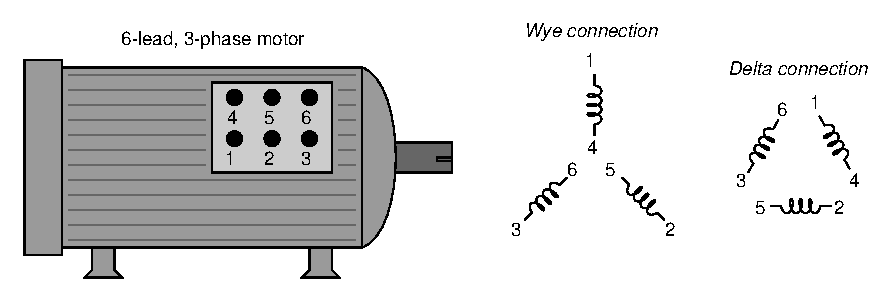
\includegraphics[width=15.5cm]{i03870x01.eps}$$

A ``Start'' contactor sends power to the stator windings in a wye configuration for a short start-up time (perhaps 10 seconds), then that starter disengages and a ``Run'' starter energizes to send power to the stator windings in a delta configuration.  In the ``wye'' configuration, each winding receives $1 \over \sqrt{3}$ of the line voltage.  In the ``delta'' configuration, each winding receives the full line voltage.

\vskip 10pt

Sketch the proper wire connections to create just such a ``wye-delta'' motor starter.  Hint: terminals 1, 2, and 3 of the motor {\it always} connect to the three-phase power lines!

$$\includegraphics[width=15.5cm]{i03870x02.eps}$$

\vskip 20pt \vbox{\hrule \hbox{\strut \vrule{} {\bf Suggestions for Socratic discussion} \vrule} \hrule}

\begin{itemize}
\item{} Explain the purpose of using reduced-voltage starting for a large electric motor.
\end{itemize}

\underbar{file i03870}
%(END_QUESTION)





%(BEGIN_ANSWER)

$$\includegraphics[width=15.5cm]{i03870x03.eps}$$

%(END_ANSWER)





%(BEGIN_NOTES)


%INDEX% Final Control Elements, motor: wye-delta starting

%(END_NOTES)

